% Resultate
\section{Resultate}

\kort{} besteht aus fünf verschiedenen Hauptmasken.
Diese sind in der Applikation über die Tabs im unteren Bereich erreichbar.

\subsection{Maske: Aufträge}
In dieser Maske werden dem Benutzer alle noch nicht gelösten Fehler in seiner Umgebung als Markierungen auf der Karte angezeigt (siehe Abbildung \ref{maske-auftraege}).
Die Fehleranzahl ist dabei auf die 25 nächstgelegenen Fehler limitiert.

Beim Klick auf einen Fehler wird der Benutzer gefragt, ob er diesen auch wirklich lösen kann.
Bestätigt er, wird ihm der Fehler im Detail angezeigt.
In dieser Detailansicht wir ihm zudem je nach Fehlertyp ein Text- oder ein Auswahlfeld angezeigt, in welchem er die Antwort eingeben bzw. auswählen kann. 

Zusätzlich gibt es die Möglichkeit, sich den Fehler nochmals auf der Karte anzuzeigen zu lassen.
Dieser wird dabei als Geometrie-Objekt angezeigt.
Eine Strasse wird dabei beispielsweise als Linie oder ein Gelände als Polygon dargestellt.

\begin{figure}[H]
\subfigure{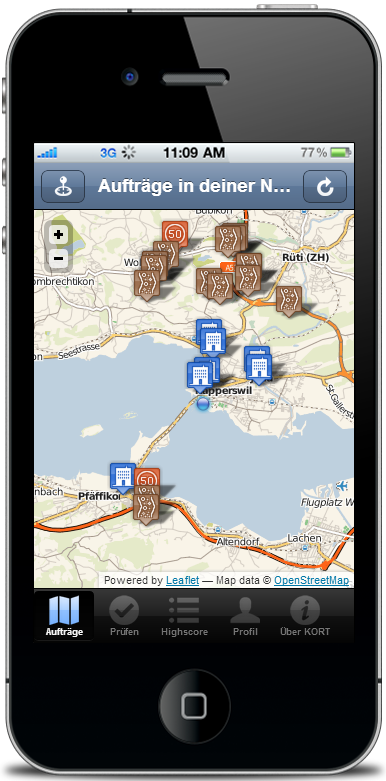
\includegraphics[width=0.3\textwidth]{images/screenshots/kort-screenshot-bugmap}}
\hfill
\subfigure{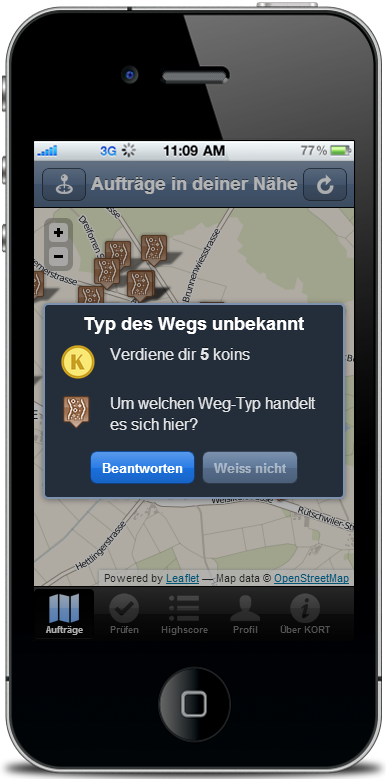
\includegraphics[width=0.3\textwidth]{images/screenshots/kort-screenshot-bugmap_message_box}}
\hfill
\subfigure{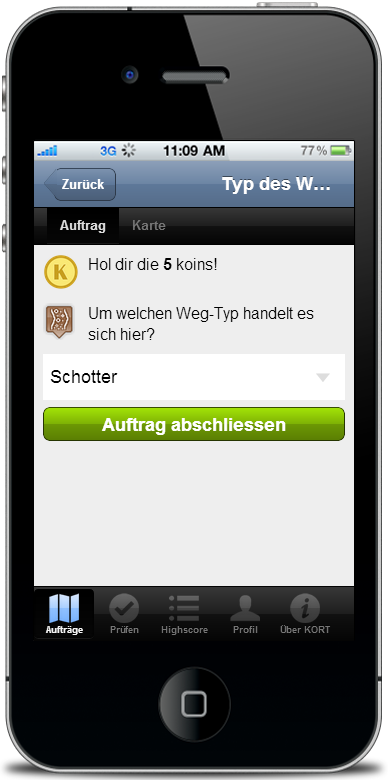
\includegraphics[width=0.3\textwidth]{images/screenshots/kort-screenshot-fix}}
\caption{Maske: Aufträge}
\label{maske-auftraege}
\end{figure}

\subsection{Maske: Prüfen}
In der \emph{Prüfen}-Maske werden dem Benutzer die Lösungen angezeigt, welche noch zu überprüfen sind (siehe Abbildung \ref{maske-pruefen}).
Diese sind dabei nach der Anzahl noch nötiger Überprüfungen gruppiert.
So soll erreicht werden, dass Lösungen, die schon bald an \brand{OpenStreetMap} zurückgesendet werden können, bevorzugt behandelt werden.
In der Liste werden maximal 25 Überprüfungen angezeigt.

Sobald der Benutzer einen Eintrag auswählt, wird ihm neben der eingetragenen Lösung auch der Fehler auf der Karte angezeigt.
Er kann nun beurteilen, ob diese Lösung korrekt oder falsch ist.

\begin{figure}[H]
\subfigure{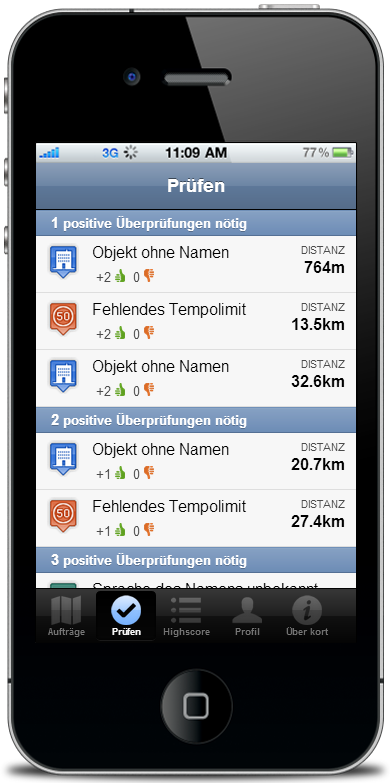
\includegraphics[width=0.3\textwidth]{images/screenshots/kort-screenshot-validation}}
\hfill
\subfigure{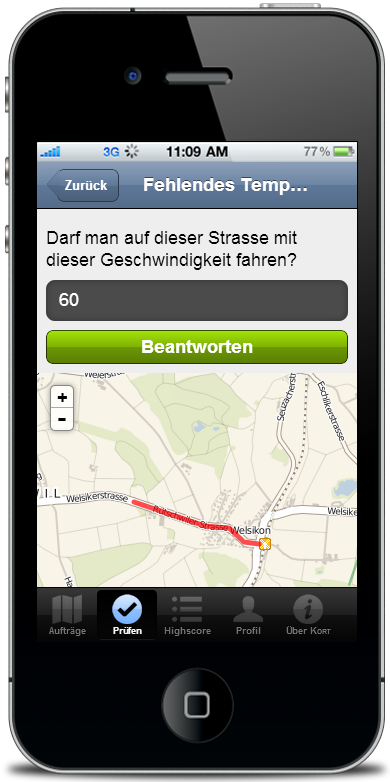
\includegraphics[width=0.3\textwidth]{images/screenshots/kort-screenshot-vote}}
\hfill
\subfigure{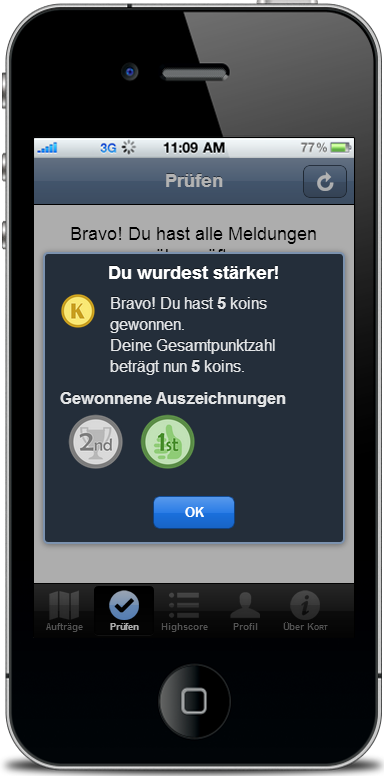
\includegraphics[width=0.3\textwidth]{images/screenshots/kort-screenshot-reward}}
\caption{Maske: Prüfen}
\label{maske-pruefen}
\end{figure}

\subsection{Maske: Highscore}
In der Highscore werden die Benutzer nach Anzahl gewonnener Punkte (sog. \emph{Koins}) sortiert (siehe Abbildung \ref{masken-highscore-profile-about}).
Es werden jeweils die ersten zehn Platzierungen angezeigt.

Wird ein Eintrag in der Highscore-Liste ausgewählt, so kann man sich das Profil des jeweiligen Benutzers anschauen.

\subsection{Maske: Profil}
Im Profil findet man eine Zusammenfassung seiner persönlichen Spielaktivitäten.
Man sieht die Gesamtanzahl der gesammelten \emph{Koins} und eine Übersicht der gewonnen Auszeichnungen (siehe Abbildung \ref{masken-highscore-profile-about}).

Auf der Profilseite lassen sich die Auszeichnungen auch in Grossformat anzeigen.

\subsection{Maske: Über Kort}
Auf der \emph{Über Kort}-Seite werden allgemeine Informationen zur Applikation angezeigt (siehe Abbildung \ref{masken-highscore-profile-about}).

\begin{figure}[H]
\subfigure{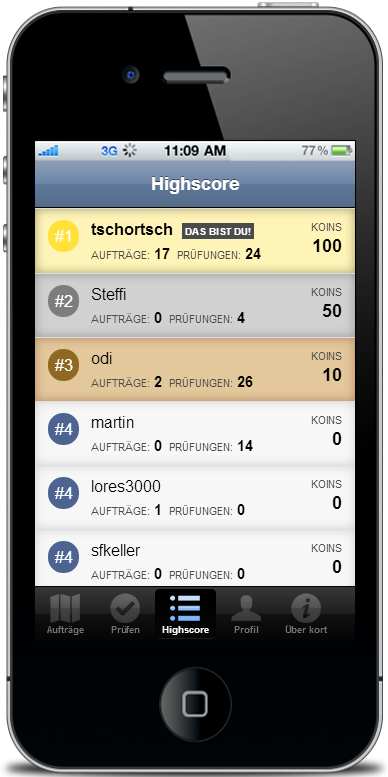
\includegraphics[width=0.3\textwidth]{images/screenshots/kort-screenshot-highscore}}
\hfill
\subfigure{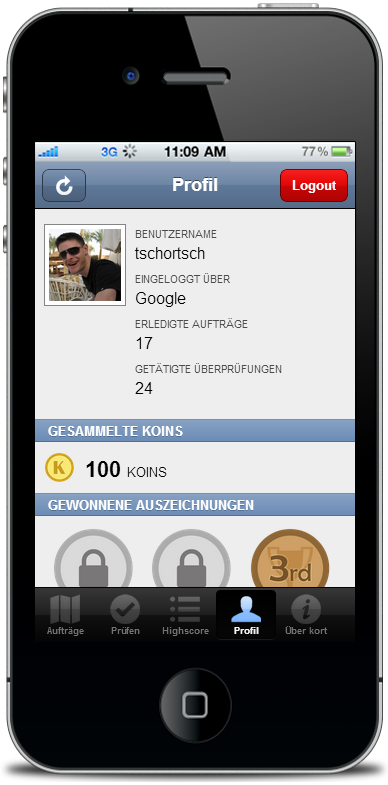
\includegraphics[width=0.3\textwidth]{images/screenshots/kort-screenshot-profile}}
\hfill
\subfigure{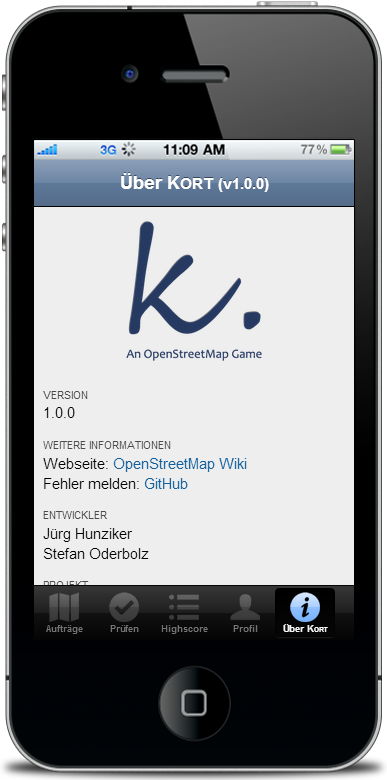
\includegraphics[width=0.3\textwidth]{images/screenshots/kort-screenshot-about}}
\caption{Masken: Highscore / Profil / Über \kort{}}
\label{masken-highscore-profile-about}
\end{figure}